\documentclass[10pt,aspectratio=43]{beamer}

\usepackage{graphicx}
\usepackage{tikz}
\usepackage{xcolor}
\usepackage{caption}
\usepackage{subcaption}
\usepackage{bm}
\usetikzlibrary{calc} 
\usepackage{hyperref}
\hypersetup{
    colorlinks=true,
    linkcolor=blue,
    urlcolor=red
}
\usepackage{fontawesome5}
\usepackage{ulem}
\usepackage[dvipsnames]{xcolor}

\usetheme{MyStyle}   % loads beamerthemeMyStyle.sty
\setlength{\columnsep}{0pt}


%%%%%%%%%%%%%%%%%%%%%%%%%%%%%%%%%%%%%%%%%%
%%%%%%%%%%%%%%%%%%%%%%%%%%%%%%%%%%%%%%%%%%
%%%%%%%%%%%%%%%%%%%%%%%%%%%%%%%%%%%%%%%%%%

\title{Electron VZ calibration \\over the run period}
\newcommand{\eventname}{ALERT meeting}
\author{Felix Touchte Codjo}
\institute{IJCLab}
\date{July 6, 2026}


\begin{document}

\begin{frame}[plain] % remove header, footer, barre de navigation
\titlepage
\end{frame}

%\begin{frame}{Outline}
%\tableofcontents
%\end{frame}

%\section{Intro}
\section{Updates}

\begin{frame}{Reminder - electron vertex in AHDC}
    \begin{itemize}
        \item We use the electron vertex in the AHDC reconstruction
    \end{itemize}

    \begin{center}
        (AHDC vz) $=$ {\color{green!50!black} (CLAS electron vz)} $-$ {\color{blue}(vz shift)}
    \end{center}

    \begin{itemize}
        \item According to the survey {\color{blue}(vz shift)} is -39.94 mm far from the center of CLAS
        \item However, looking at the timeline, we know that the vz reconstruction might be bias depending on the torus configuration
            \begin{itemize}
                \item up to 30 mm shift between the inbending and outbending configuration
            \end{itemize}
        \item We decide to determine {\color{blue}(vz shift)} empirically
    \end{itemize}

    \centering
    \vspace{0.2cm}

    \begin{figure}
        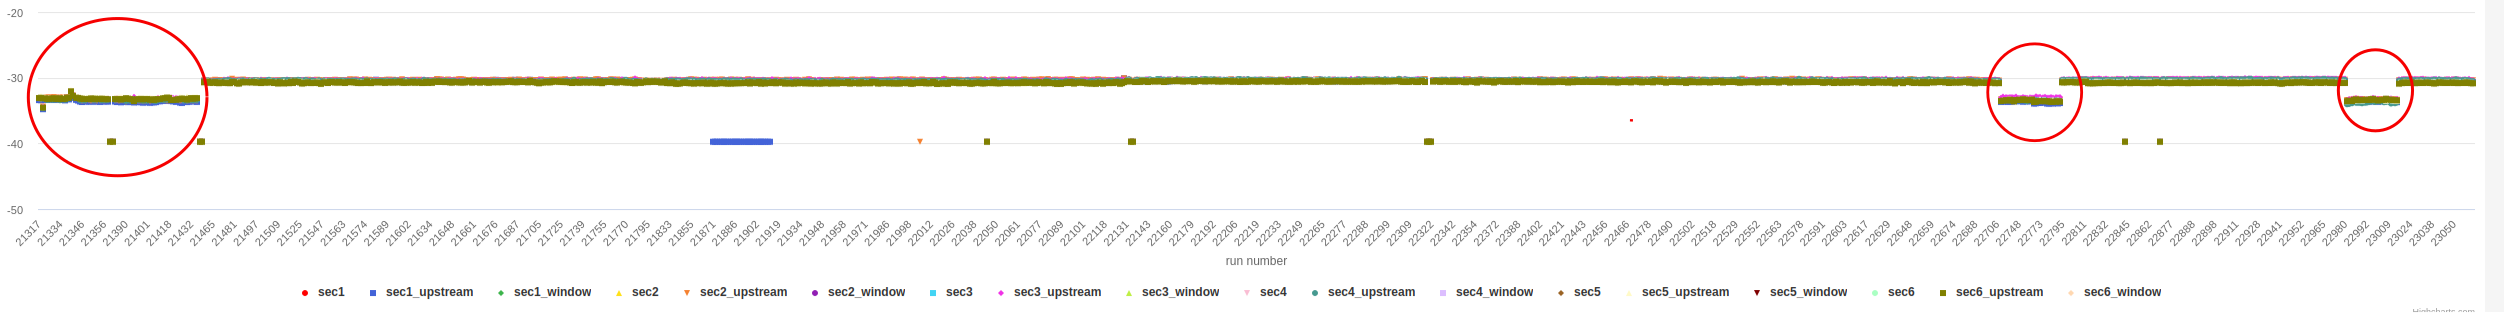
\includegraphics[width=\linewidth]{figures/upstream_vz_peak_over_run.png}
        \caption{Forward electron vz (upstream peak value). See \href{https://clas12mon.jlab.org/rgl/pass0_v10.3_alert/forward/timeline/}{timeline}}
    \end{figure}

\end{frame}


\begin{frame}{vz alignment}
    \begin{itemize}
        \item principle : {\color{green!50!black} (CLAS electron vz)} $-$  (AHDC vz) $-$ {\color{blue}(vz shift)} should be zero
        \item Outbending (left column), Inbending (right column)
        \item The optimal values are -67 mm and -36 mm
    \end{itemize}

    \centering
    \vspace{0.2cm}

    \begin{tabular}{cc}
        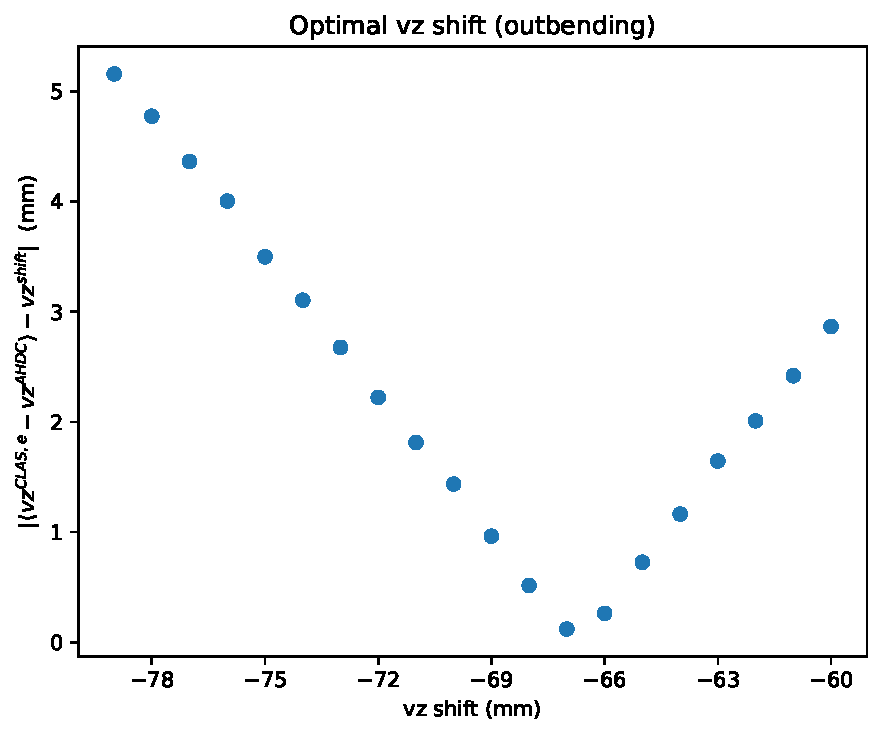
\includegraphics[width=0.34\linewidth]{figures/delta_value_2gev.pdf}    & 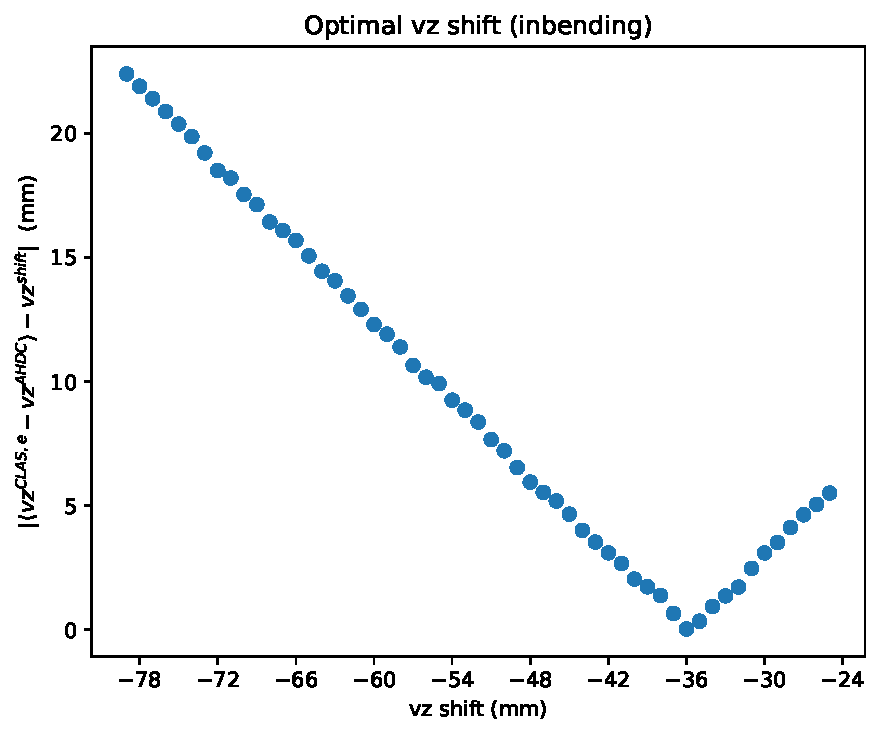
\includegraphics[width=0.34\linewidth]{figures/delta_value_10gev.pdf} \\
        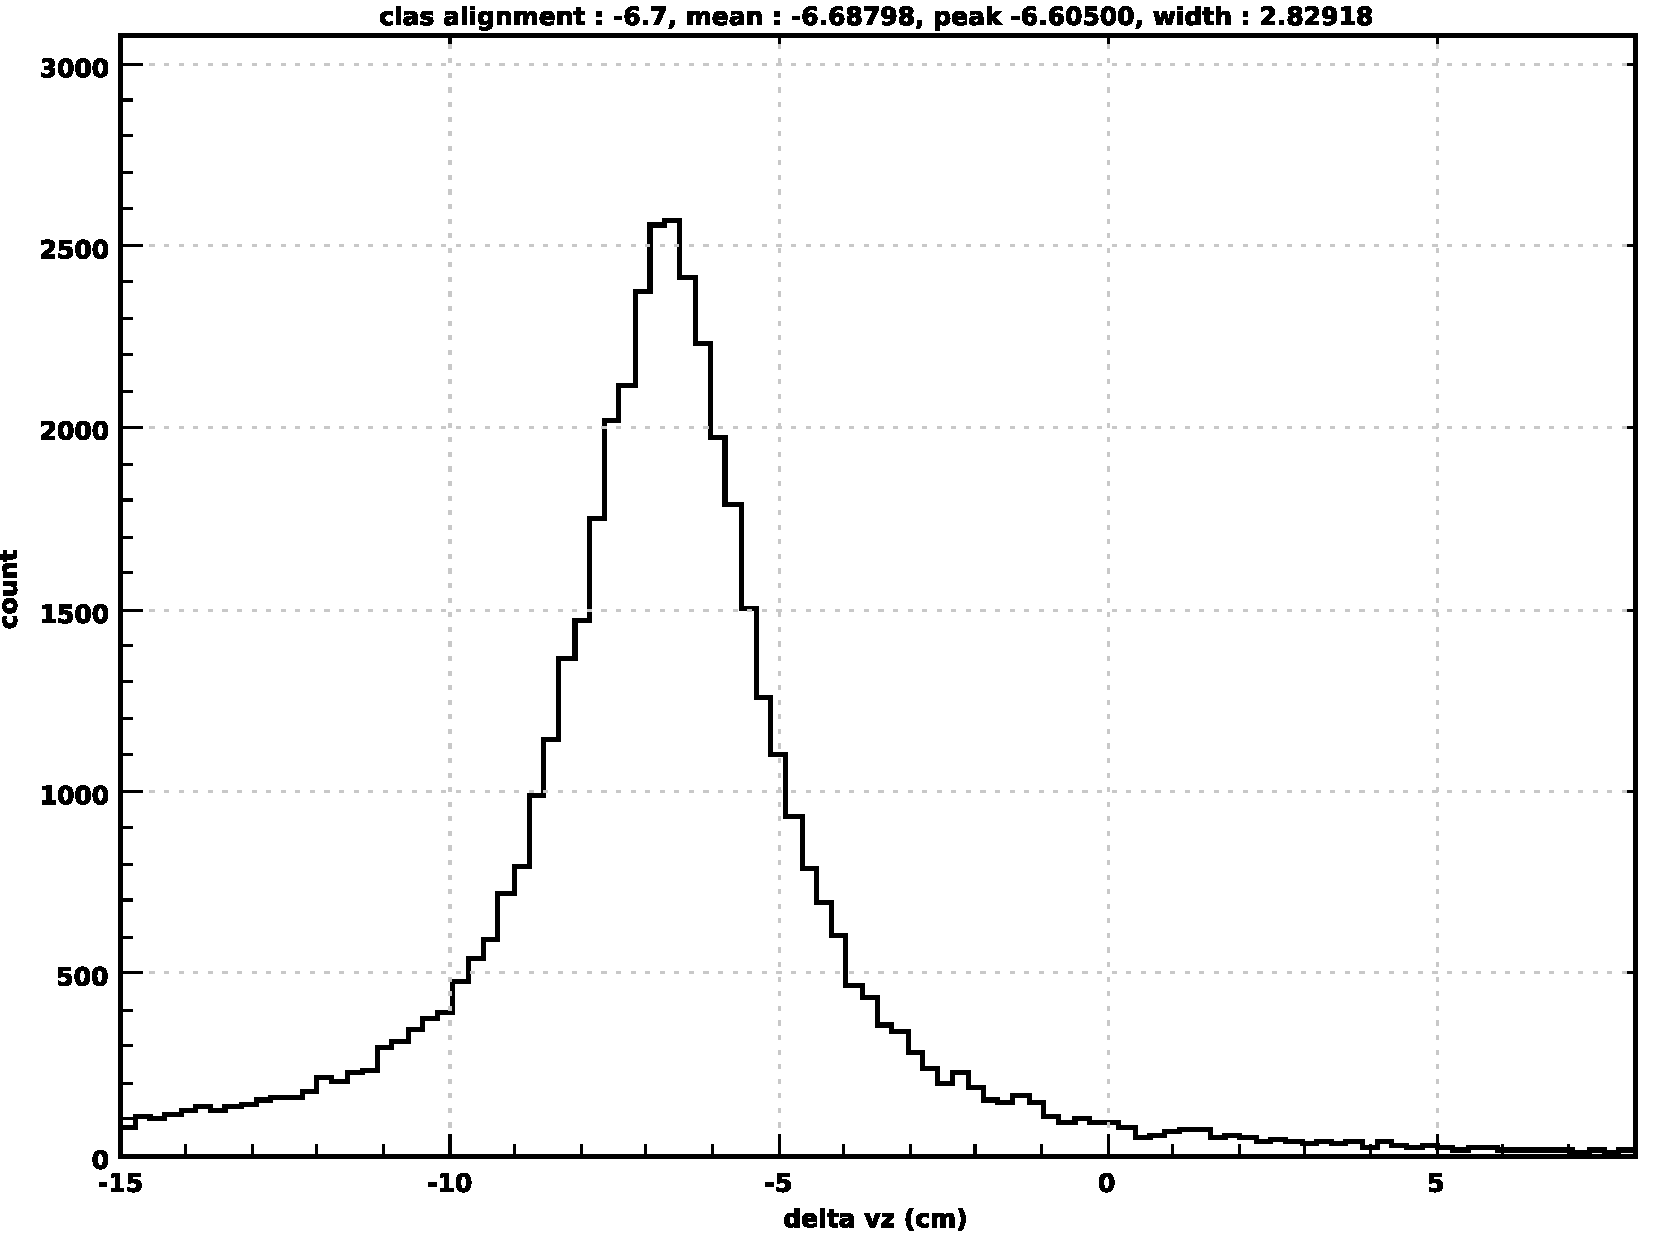
\includegraphics[width=0.34\linewidth]{figures/track_delta_vz_2gev.pdf} & 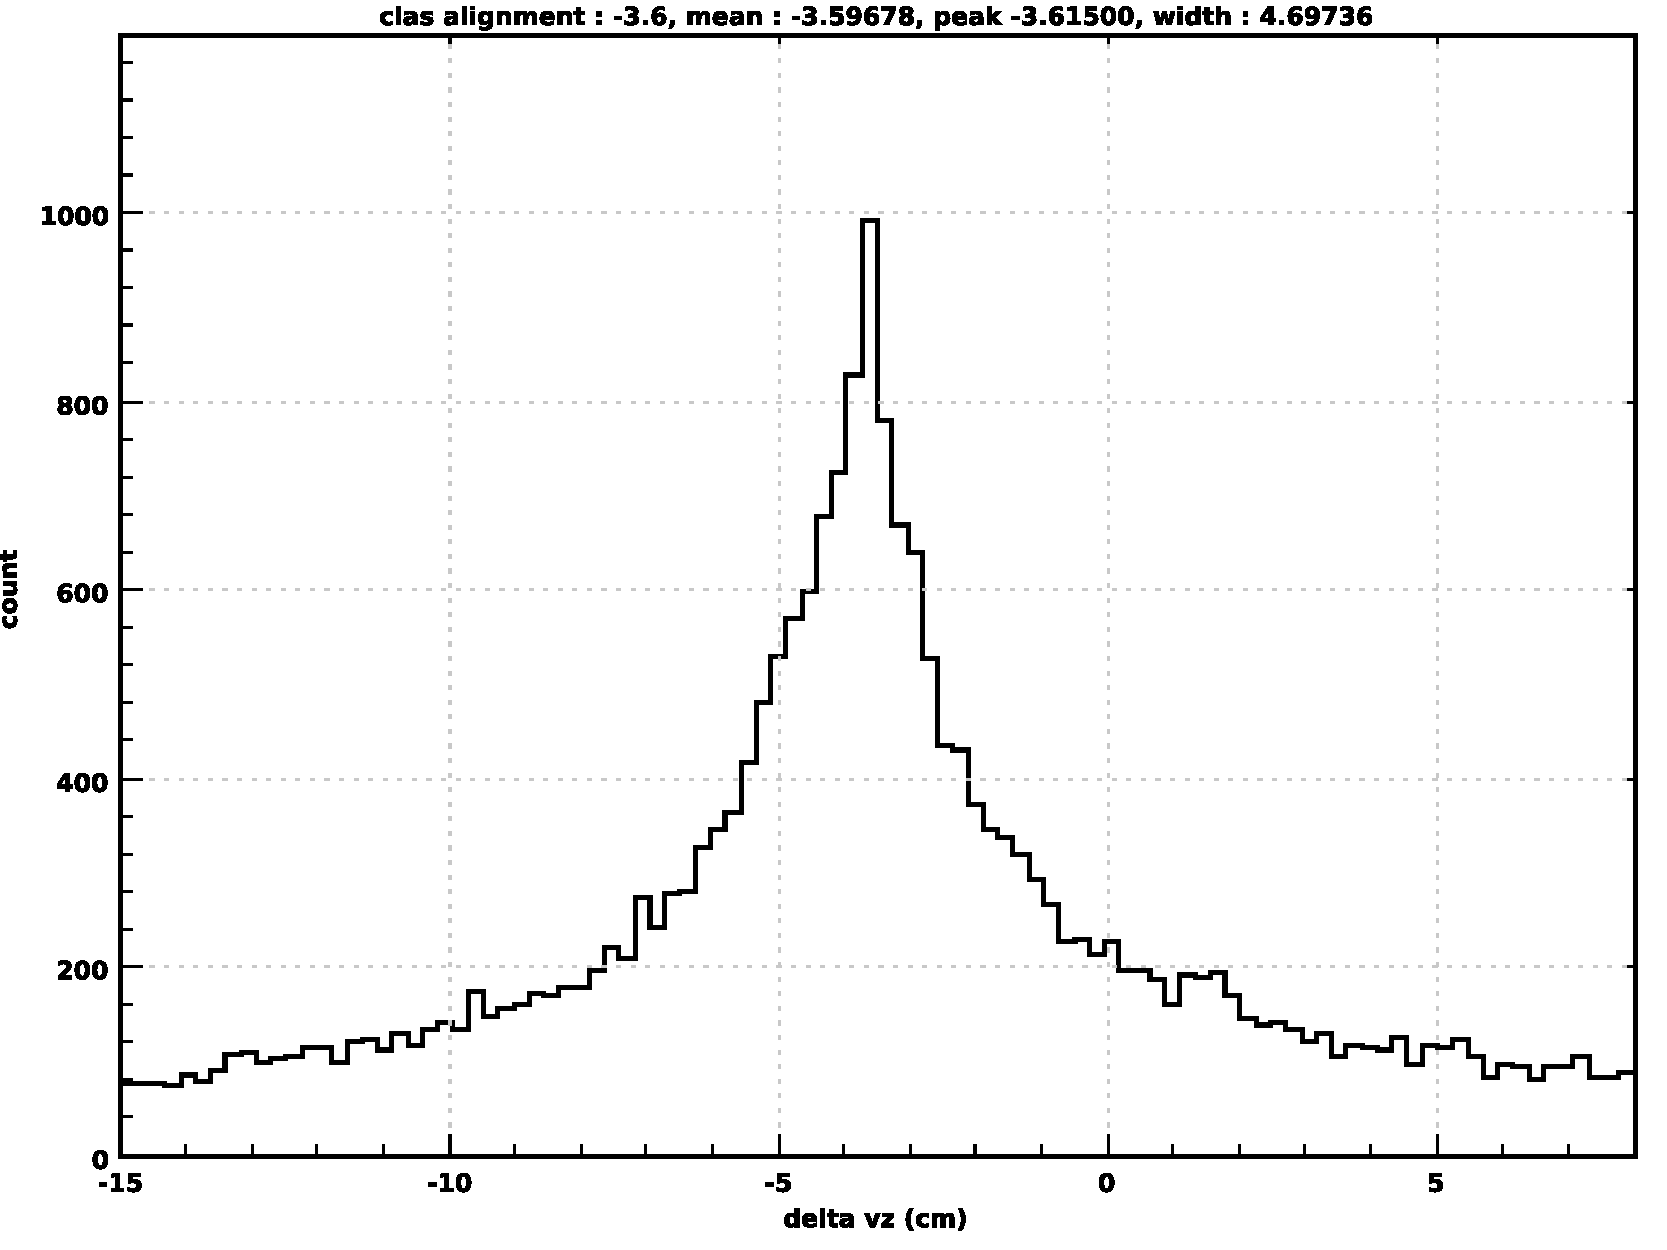
\includegraphics[width=0.34\linewidth]{figures/track_delta_vz_10gev.pdf} \\
    \end{tabular}
\end{frame}

\begin{frame}{Backup slides}
    \begin{itemize}
        \item Outbending $\rightarrow$ 2.24 GeV data $\rightarrow$ elastic cuts : $3.5 < W^2 < 3.8 \mbox{ GeV}^2$, $\Delta \phi < \mbox{20}^\circ$, nhits $>$ 6
        \item Inbending $\rightarrow$ 10.6 GeV data $\rightarrow$ nhits $>$ 6, chi2 $<$ 8, no FT electron
        \item The upstream VZ peak (the one located on the left) vary over the run period. This is mainly due to the change of the torus configuration
    \end{itemize}

    \centering
    \vspace{0.2cm}

    \begin{figure}
        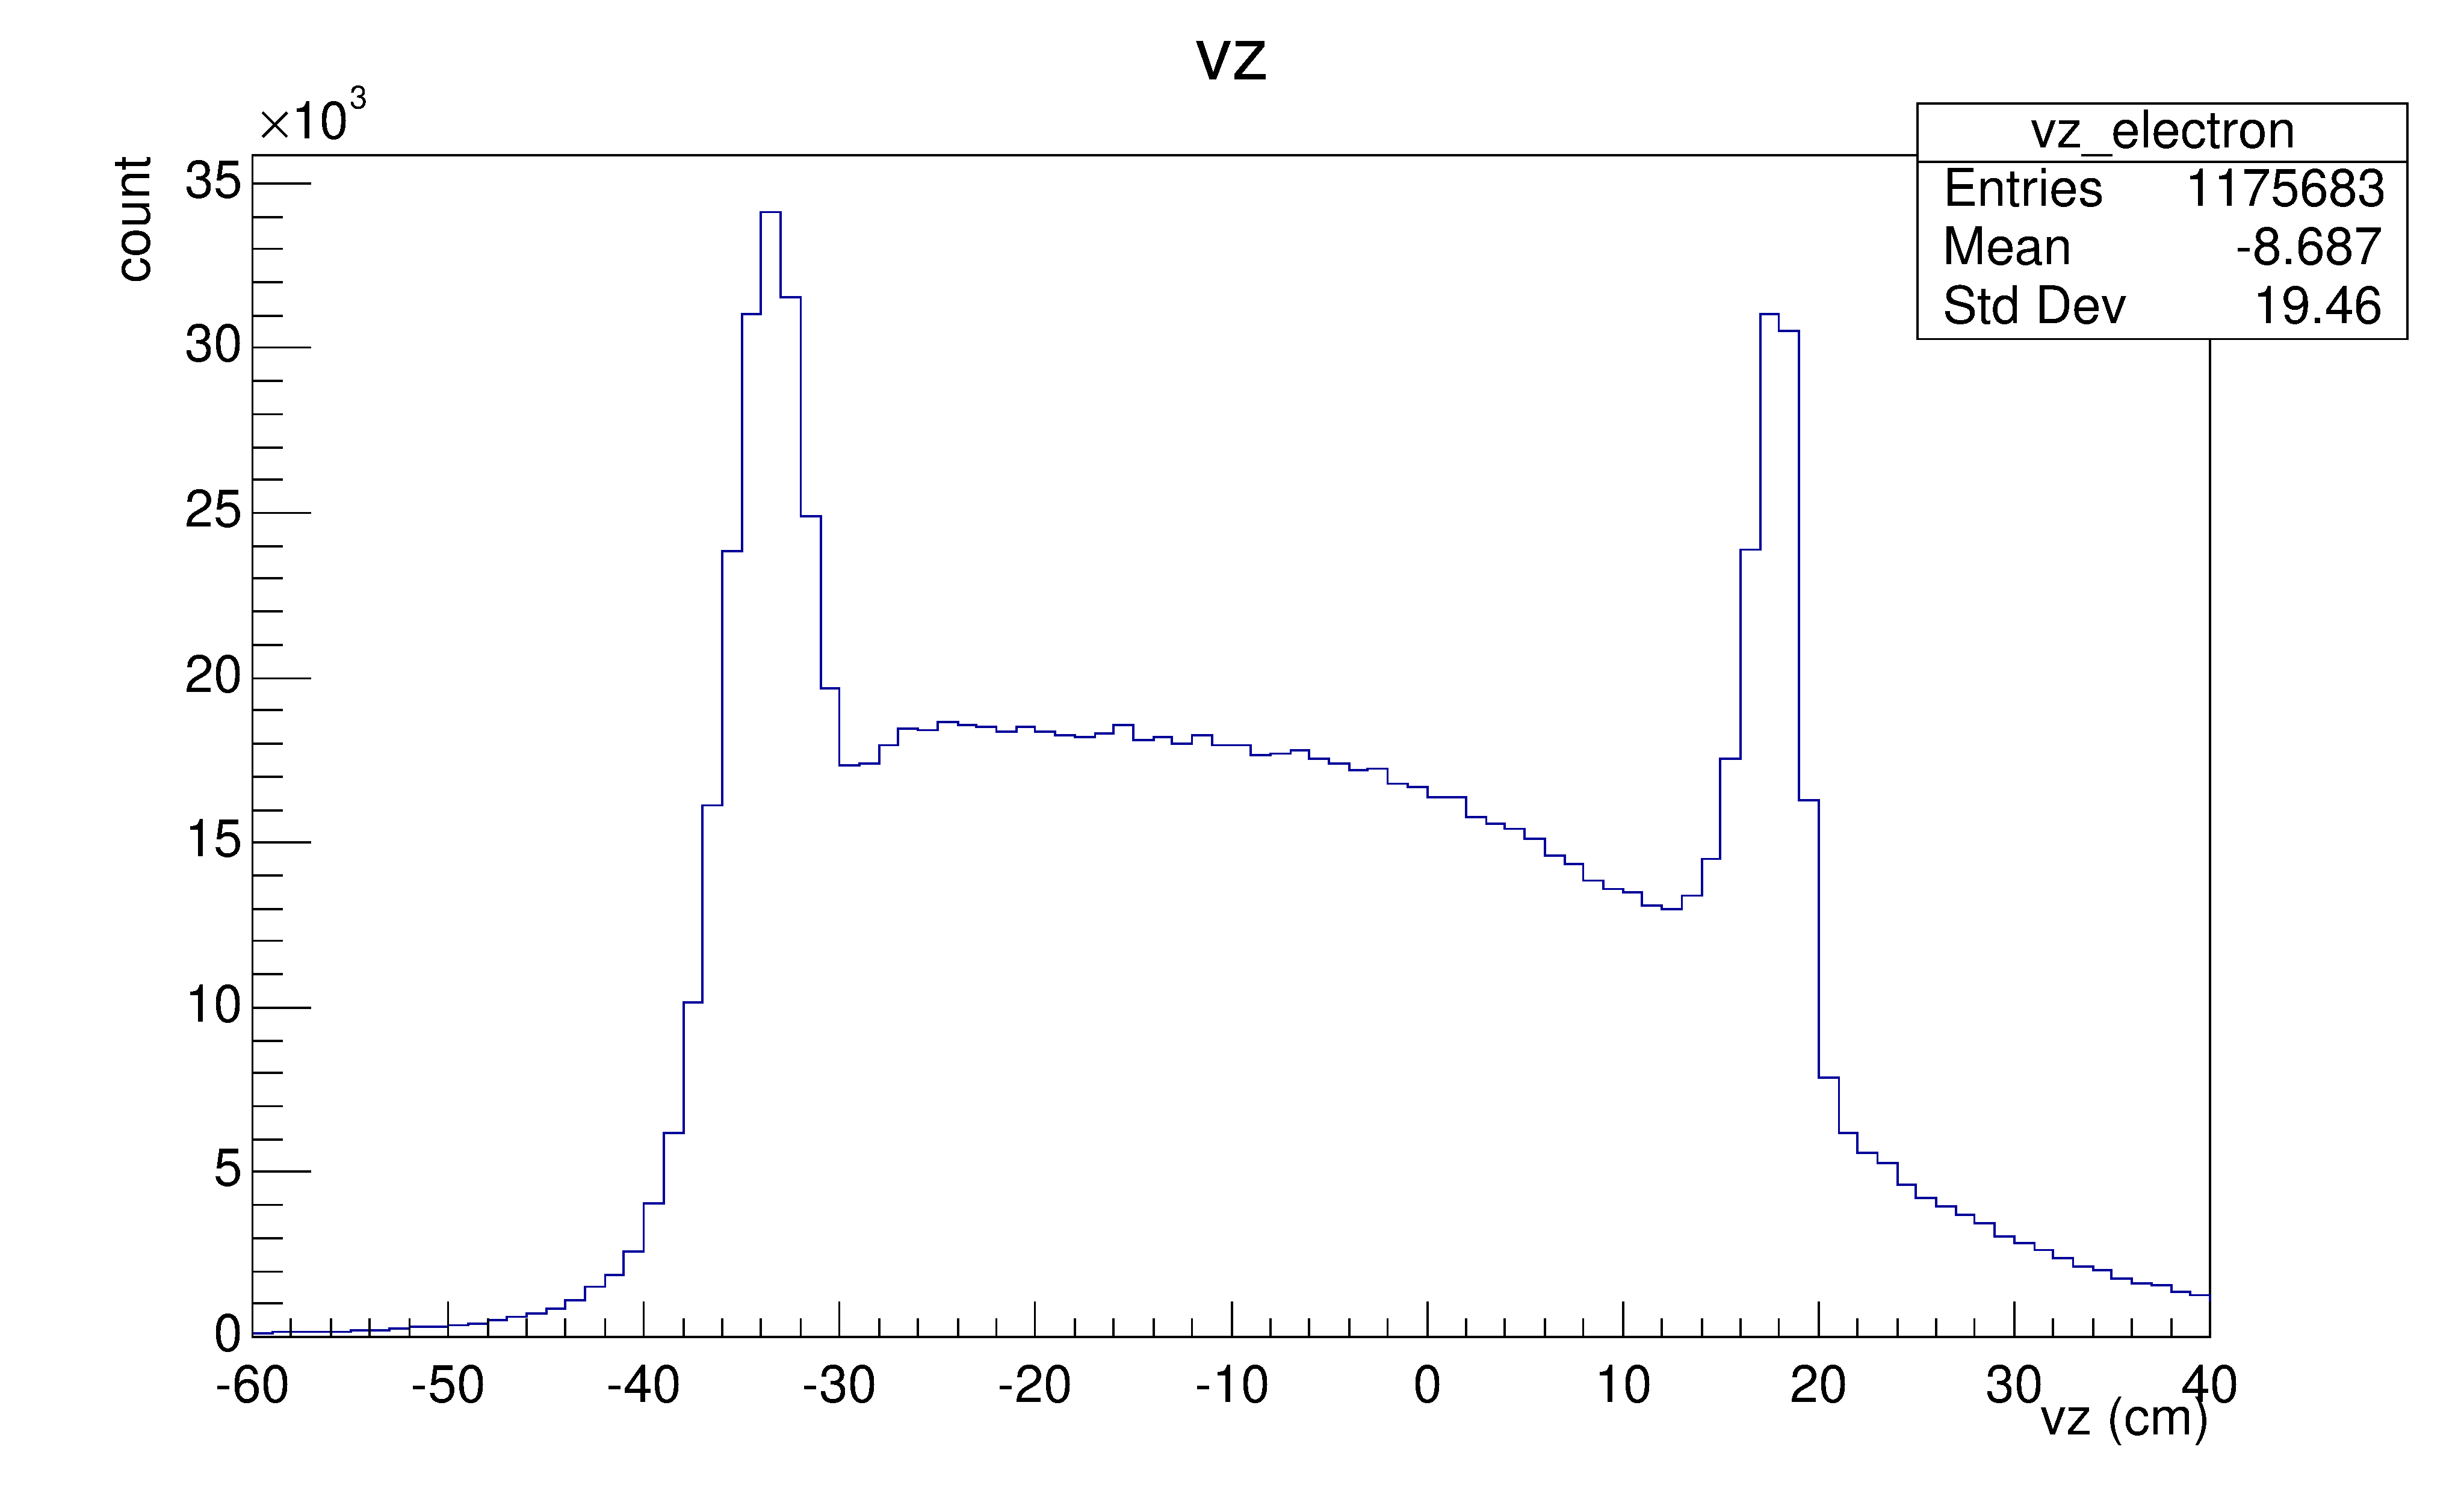
\includegraphics[width=0.6\linewidth]{figures/alignment_forward_vz_electron.pdf}
        \caption{CLAS electron vertex. Run 22712 (outbending config).}
    \end{figure}

    
\end{frame}







\end{document}


